\section{Coloured Petri Nets}
\label{sec:cpn}
One way to approach the challenge of building concurrent systems is to build a formal model, e.g., a Coloured Petri Net (CPN) \cite{RefWorks:3} model. Constructing and simulating an executable model gives insight into the system being modelled and reveals errors. Furthermore, building the model often leads to a more complete specification. A CPN model of a system describes the state and the events that can change the state of the system. The model can be simulated which enables the developer to investigate the system through different scenarios.

% Producer-consuming example description
We explain the CPN language through a producer-consumer system which will be the running example throughout this thesis. In our producer-consumer system two different kinds of entities are running concurrently:	

\begin{itemize}
  \item $n$ producers run simultaneously. A producer alternates between producing and sending data to a consumer. 
  \item $m$ consumers run simultaneously. A consumer alternates between receiving data from a producer and consuming data.  
\end{itemize} 

The data produced, send, received, and consumed is represented as integers. Producers can send the produced data to a specific consumer determined by the value of a global variable. In section~\ref{sec:validateprodcons} we introduce a load-balancer which can change the value of this global variable.

\begin{figure}[b!]
\centering
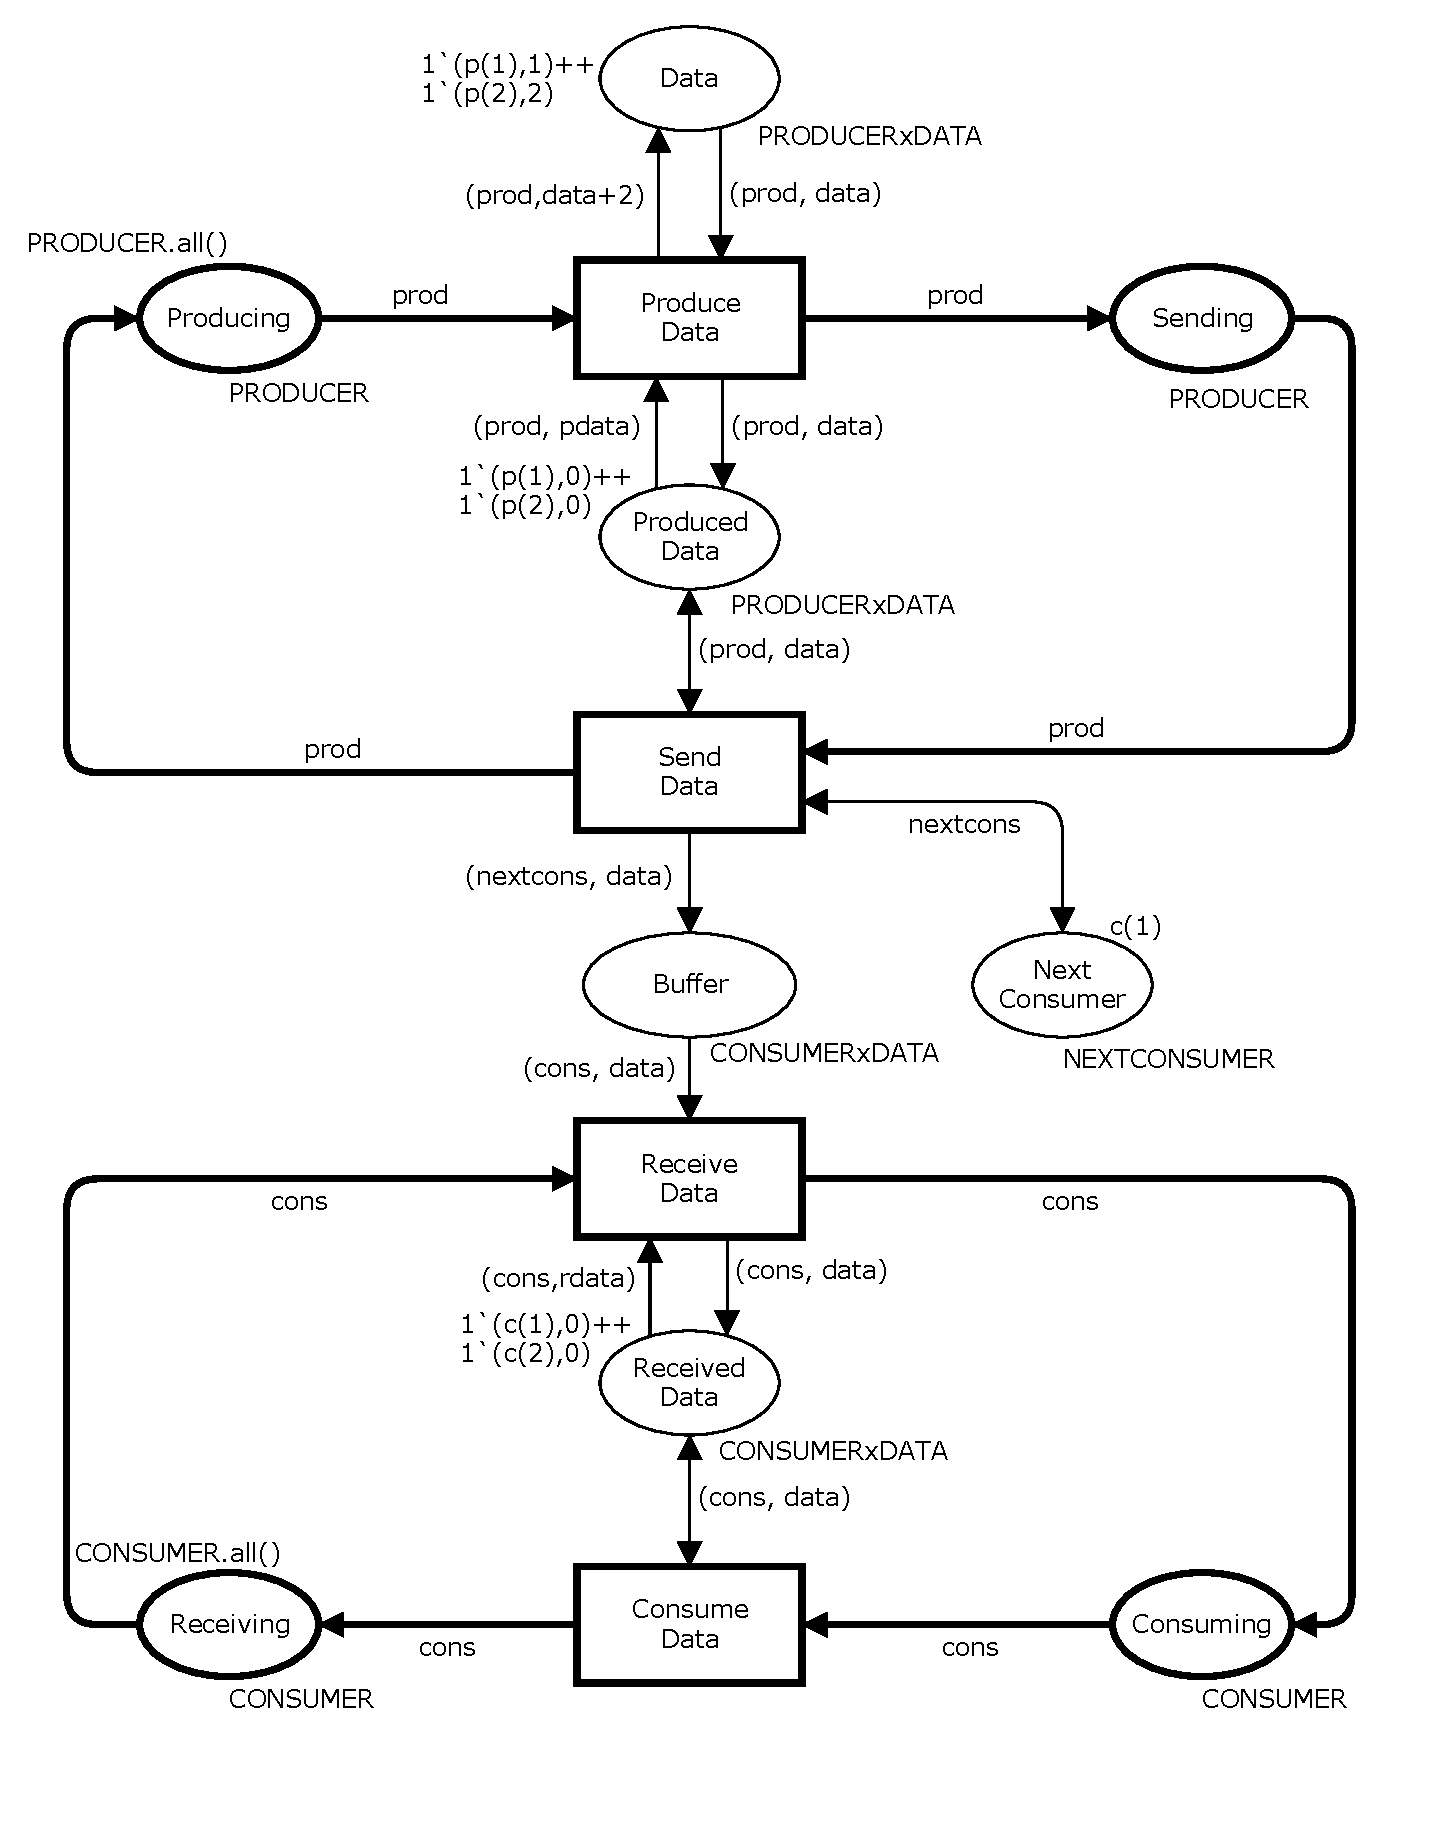
\includegraphics[scale=0.5]{background/graphics/System.eps}
\caption{The producer-consumer CPN model}
\label{fig:systemmodule}
\end{figure}

% The producer-consumer CPN model
A graphical drawing of the CPN model is shown in Fig. \ref{fig:systemmodule}. The top part models the producers and the bottom part models the consumers. The CPN model contains nine \emph{places} (drawn as ellipses), four \emph{transitions} (drawn as rectangular boxes), a number of directed \emph{arcs} connecting places and transitions, and finally some textual \emph{inscriptions} next to the places, transitions and arcs. The inscriptions are written in an extension of the Standard ML language called \emph{CPN ML}. Places and transitions are called \emph{nodes} and together with the arcs they constitutes the \emph{net structure}. An arc either connects a transition to a place or a place to a transition. Thus it is illegal to, e.g., connect a place to another place.  

% Places
The places represent the state of the modelled system. Each place has a number (possibly zero) of tokens, and each token has a data value (called a \emph{token colour}) attached to it. The \emph{marking} of a specific place is the number of tokens and their colour on that place. The marking of the entire CPN model is described by the union of the markings of each place in the model. The state of the producers is described by the four places \figitem{Producing}, \figitem{Sending}, \figitem{Data}, and \figitem{ProducedData}. The state of the consumers is described by the three places \figitem{Receiving}, \figitem{Consuming} and \figitem{ReceivedData}. 

Each place has a type inscription, called the \emph{colour set}, that specifies which token colours are allowed on that place. The colour set keyword in CPN ML is simply \code{colset}. The colour set at the places \figitem{Producing} and \figitem{Sending} is \code{PRODUCER}, and the colour set at the places \figitem{Receiving} and \figitem{Consuming} is \code{CONSUMER}, which are defined:

\begin{verbatim}
colset PRODUCER = index p with 1..2;
colset CONSUMER = index c with 1..2;
\end{verbatim}

\noindent
Both \code{PRODUCER} and \code{CONSUMER} are \emph{index} colour sets. Indexed values are sequences of values comprised of an identifier and an index-specifier. These colour sets are used to represent and identify the different producers and consumers. The places \figitem{Data} and \figitem{ProducedData} have the colour set:

\begin{verbatim}
colset PRODUCERxDATA = product PRODUCER * DATA; 
colset CONSUMERxDATA = product CONSUMER * DATA;
\end{verbatim}

\noindent
The \code{product} keyword is used to create tuples. Both \code{PRODUCERxDATA} and \code{CONSUMERxDATA} are two-tuples (pairs) where the first element is a producer or a consumer respectively and the second element is data.

Next to each place there is another inscription called the \emph{initial} marking. For instance, the place \figitem{Producing} has the initial marking \code{PRODUCER.all()} which specifies that the initial marking of \figitem{Producing} contains all producers. Analogously, the place \figitem{Receiving} contains all the consumers initially. The number of producers and consumers depends on the scenario investigated. In this example we have two producers and two consumers. The initial marking of the place \figitem{Data} is described by the multi-set:

\begin{verbatim}
1`(p(1), 1) ++ 1`(p(2), 2);
\end{verbatim}

\noindent
A \emph{multi-set} is a set where elements are quantified. The \code{++} and \code{`} are operators on multi-sets. The elements are quantified by the infix operator \code{`} which takes a non-negative integer as left argument and an element as right argument. For instance, \code{1`(p(1), 1)} means that there is one appearance of the element \code{(p(1), 1)}. The meaning of the pair \code{(p(1), 1)} is that we associate producer \emph{1} with the integer data element one. The multi-set infix operator \code{++} is used to take the union of two multi-sets. The places \figitem{Sending}, \figitem{ProducedData}, \figitem{Consuming} \figitem{ReceivedData} and  \figitem{Buffer} are initially empty, whereas the place \figitem{NextConsumer} contains the multi-set \code{1`c(1)}.

% Transitions 
The four transitions (drawn as rectangles) represent the events that can occur in the system. When a transition \emph{occurs} it removes tokens from \emph{input} places (those having an arc pointing towards the transition) and adds tokens to the \emph{output} places (those having arcs pointing away from the transition). For instance, when the transition \figitem{ProduceData} occurs it removes a producer token from the input place \figitem{Producing} and a data token, belonging to the same producer, from the input place \figitem{Data}. Then it adds the same producer token to the output place \figitem{Sending} and the pair associating the producer with the data to the output place \figitem{ProducedData}. 

% Arcs
The colour of a token added or removed by a transition is determined by the \emph{arc expressions} on the arcs connecting the transition to the input and output places. The arc expressions are written in the CPN ML programming language and may contain constants, typed variables, operator expressions or functions. The arc expressions are evaluated when all variables are bound to a value and evaluates to a multi-set of token colours. On an output arc the multi-set of token colours outputted by the arc expression is added to the connected output place. On an input arc the multi-set of token colours outputted by the arc expression is removed from the connected input place. As an example, consider the two arcs connecting the input places \figitem{Producing} and \figitem{Data} to the transition \figitem{ProduceData}. The two arc expressions contain the variables: 

\begin{verbatim}
var prod : PRODUCER
var data : DATA
\end{verbatim}

\noindent
This means that \code{prod} must be bound to a value of type \code{PRODUCER} and data must be bound to a value of type \code{DATA}. A valid \emph{binding} of variables could be the following binding which binds \code{prod} to producer \emph{1} and \code{data} to the integer one:

\begin{verbatim}
<prod=p(1),data=1>
\end{verbatim}


\subsection{Enabling and Occurrence of Transitions}
A transition is \emph{enabled} if the arc expressions on the \emph{input} arcs evaluates to multi-sets which is present on the input places connected to the transitions. Furthermore, the guard of the transition must evaluate to \emph{true} (guards are explained in section \ref{subsec:guards}). We then say that the transition can \emph{occur} in that marking. When the transition occurs it removes from each input place the multi-set of token colours to which the corresponding input arc evaluates. It then adds to each output place the token colours to which the corresponding output arcs evaluate.

\begin{figure}
\centering
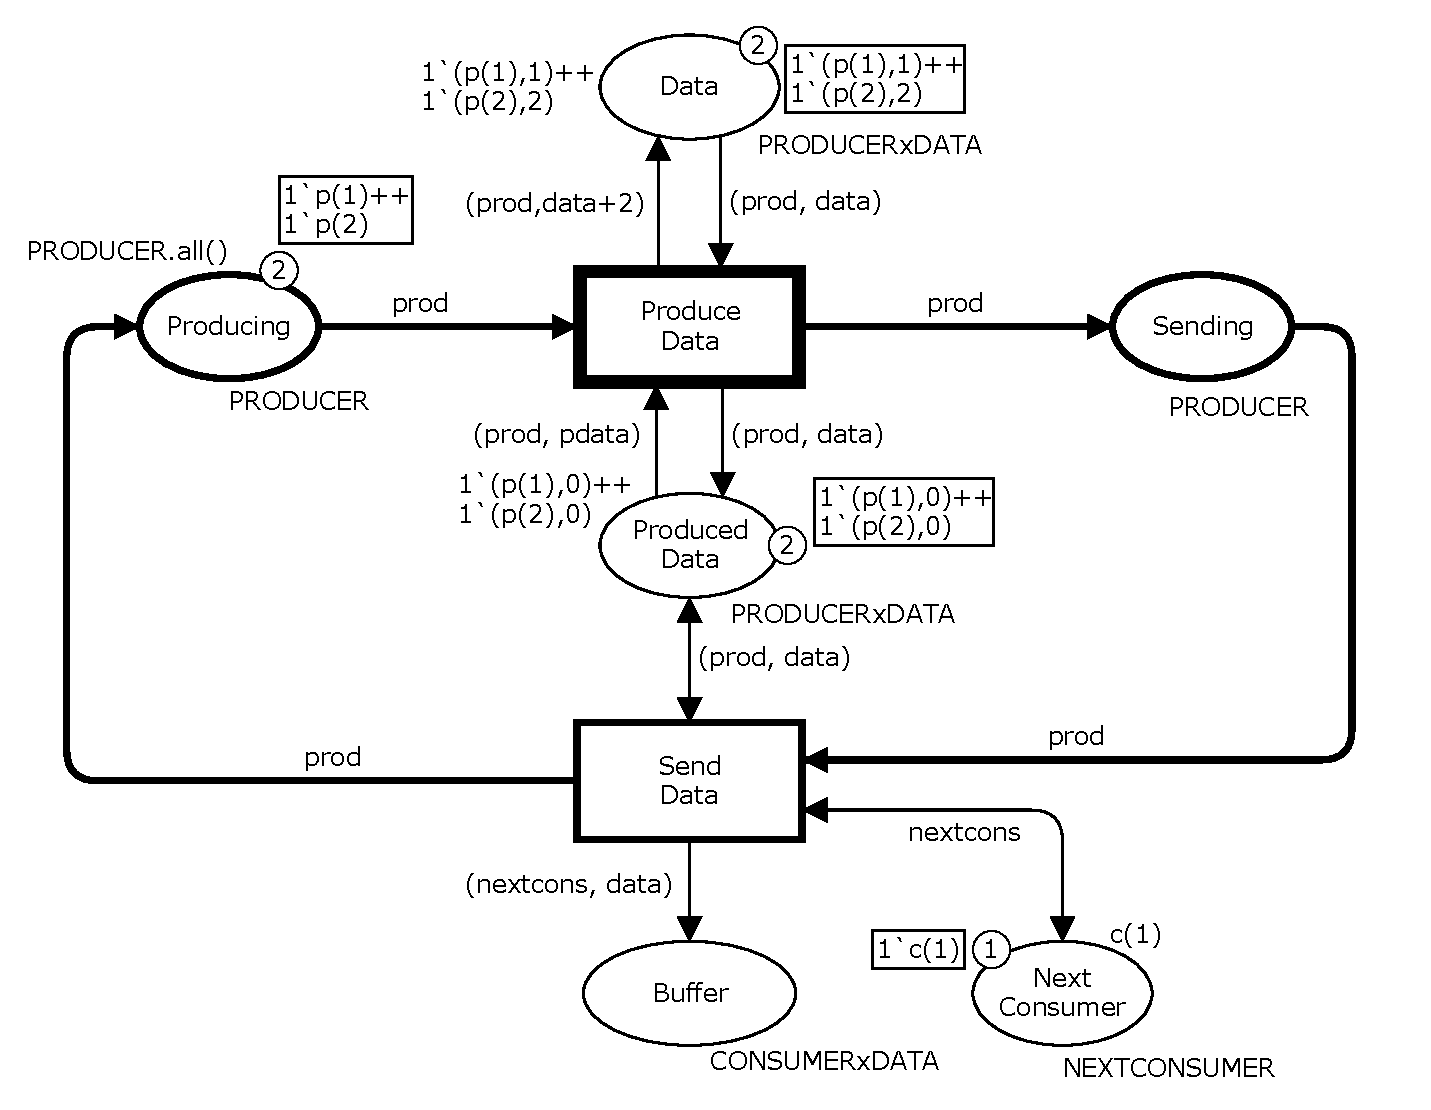
\includegraphics[scale=0.40]{background/graphics/SystemProducerM0.eps}
\caption{The initial marking $M_0$ showing the producer part of the model}
\label{fig:systemmoduleProducerM0}
\end{figure}

Let us consider Fig.~\ref{fig:systemmoduleProducerM0} in which the initial marking of the producer part of the model are shown. We see two producers on the place \figitem{Producing}. Producer \code{p(1)} has the integer data value \code{1} on the place \figitem{Data} and producer \code{p(2)} has the value \code{2}. The transition \figitem{ProduceData} has a thick border line which in CPN Tools means that the transition is enabled. The transition \figitem{SendData} is not enabled meaning it can not occur in the initial marking. There are two possible bindings for the variable \code{prod} on the input arc going from the input place \figitem{Producing} to the transition \figitem{ProduceData}. If \code{prod} is bound to \code{p(1)} the task is to find a binding of the variables on the input arc connecting the \figitem{Data} to \figitem{ProduceData} such that the arc expression evaluates to a multi-set of tokens where \code{prod=p(1)}. The resulting binding is:

\begin{verbatim}
<prod=p(1),data=1>
\end{verbatim}

\noindent
An occurrence of the transition \figitem{ProduceData} with the binding from above removes the token with colour \code{p(1)} from \figitem{Producing} and \code{(p(1),1)} from \figitem{Data}. It then adds the result of evaluating the output arc expressions, which means that a token colour \code{p(1)} is added to the place \figitem{Sending}, the pair \code{(p(1),1)} is added to the place \figitem{ProducedData} and the pair \code{(p(1),3)} is added to the place \figitem{Data}. The resulting marking $M_1$ is shown in Fig. \ref{fig:systemmoduleProducerM1} and again only the producer part of the model is shown since the marking of the consumer part is unchanged. 

\begin{figure}[b!]
\centering
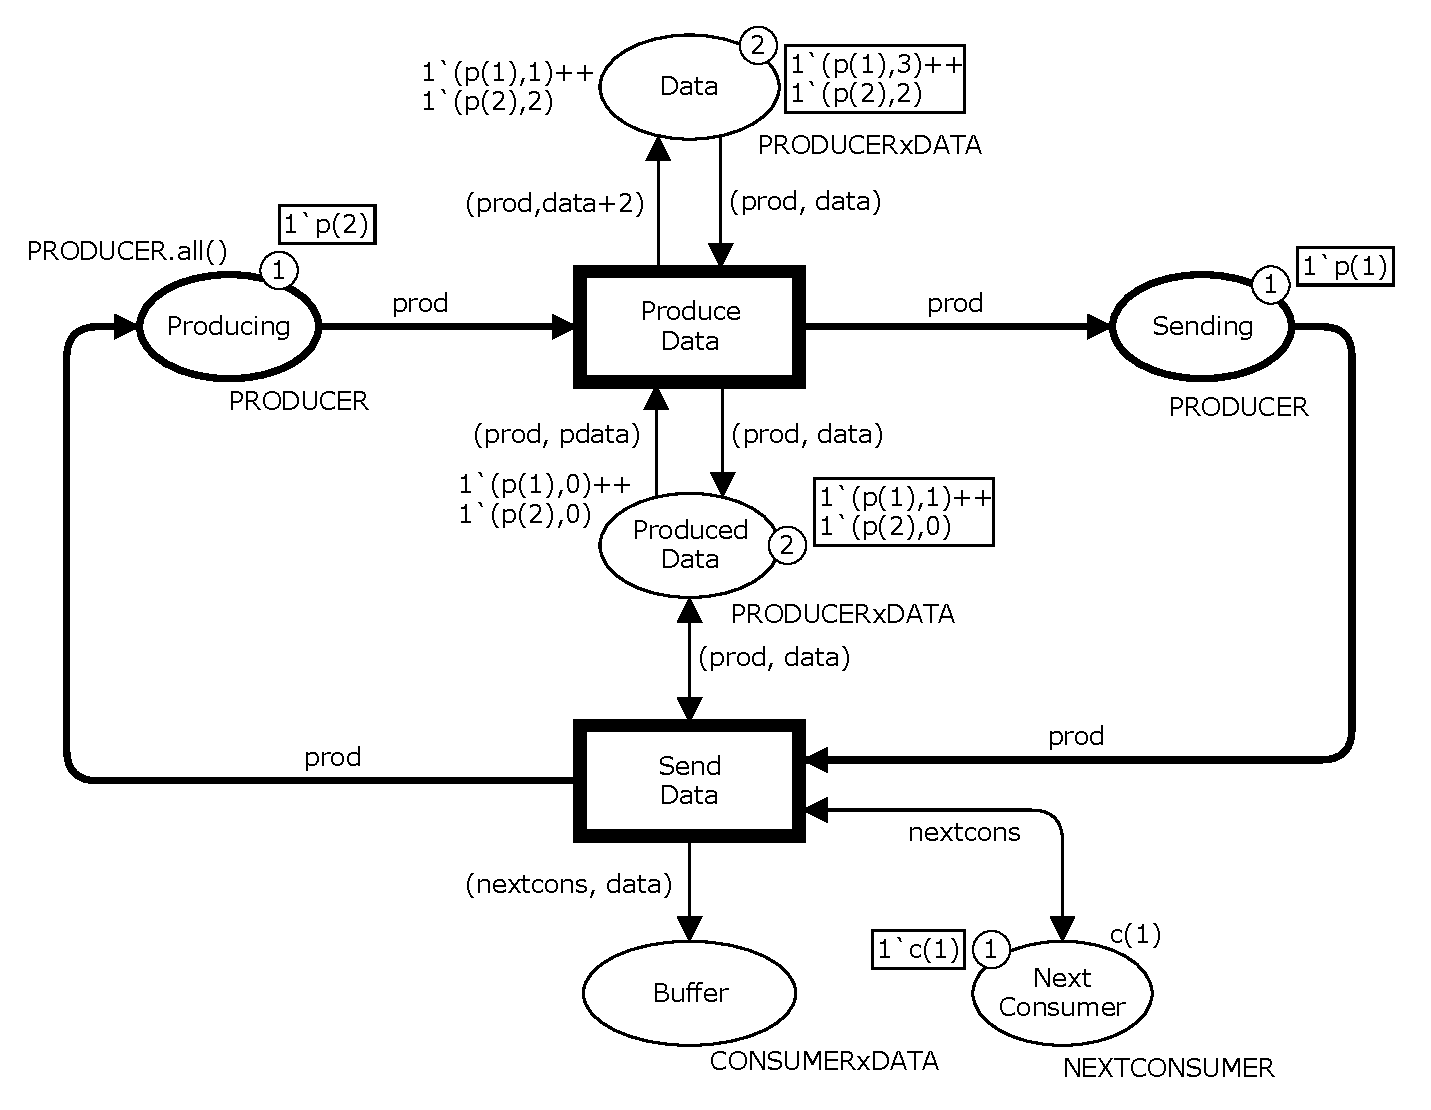
\includegraphics[scale=0.40]{background/graphics/SystemProducerM1.eps}
\caption{The producer part of the model in marking $M_1$}
\label{fig:systemmoduleProducerM1}
\end{figure}

In marking $M_1$ in Fig.~\ref{fig:systemmoduleProducerM1} we can see that the token colour \code{p(1)} now resides on the place \figitem{Sending} and that the transition \figitem{SendData} now has a thick border line indicating that it is enabled. Intuitively, this means that the producer \emph{1} is now in a sending state ready to send out the data that was just produced. 

The notation for the occurrence of a transition with a given binding is called a \emph{binding element} and is written as a pair where the first element is the transition and the second element is the binding of variables for that transition. In the marking $M_1$ there are two binding elements enabled: \\*
\newline
(\figitem{ProduceData}, \code{<prod=p(2),data=1>})\\*
(\figitem{SendData}, \code{<prod=p(1),data=1, nextcons=c(1)>})\\*
\newline
Choosing the second binding element results in adding a data element to the buffer and changing the state of producer \emph{1} back to producing. Letting this binding element occur will lead to marking $M_2$ which can be seen in Fig.~\ref{fig:systemmoduleM2}. In this marking the token \code{p(1)} is moved back to the place \figitem{Producing} and the token \code{c(1),1} is added to the place \figitem{Buffer}. This means that data can now be received by a consumer \emph{1}. Notice how the variable \code{nextcons} is used to determine the receiver of the produced data. In a sense, the place \figitem{NextConsumer} is trivial representation of a \emph{load-balancer} that never changes the receiver of the produced data. In section~\ref{sec:validateprodcons} we present a more useful load-balancer. 

\begin{figure}
\centering
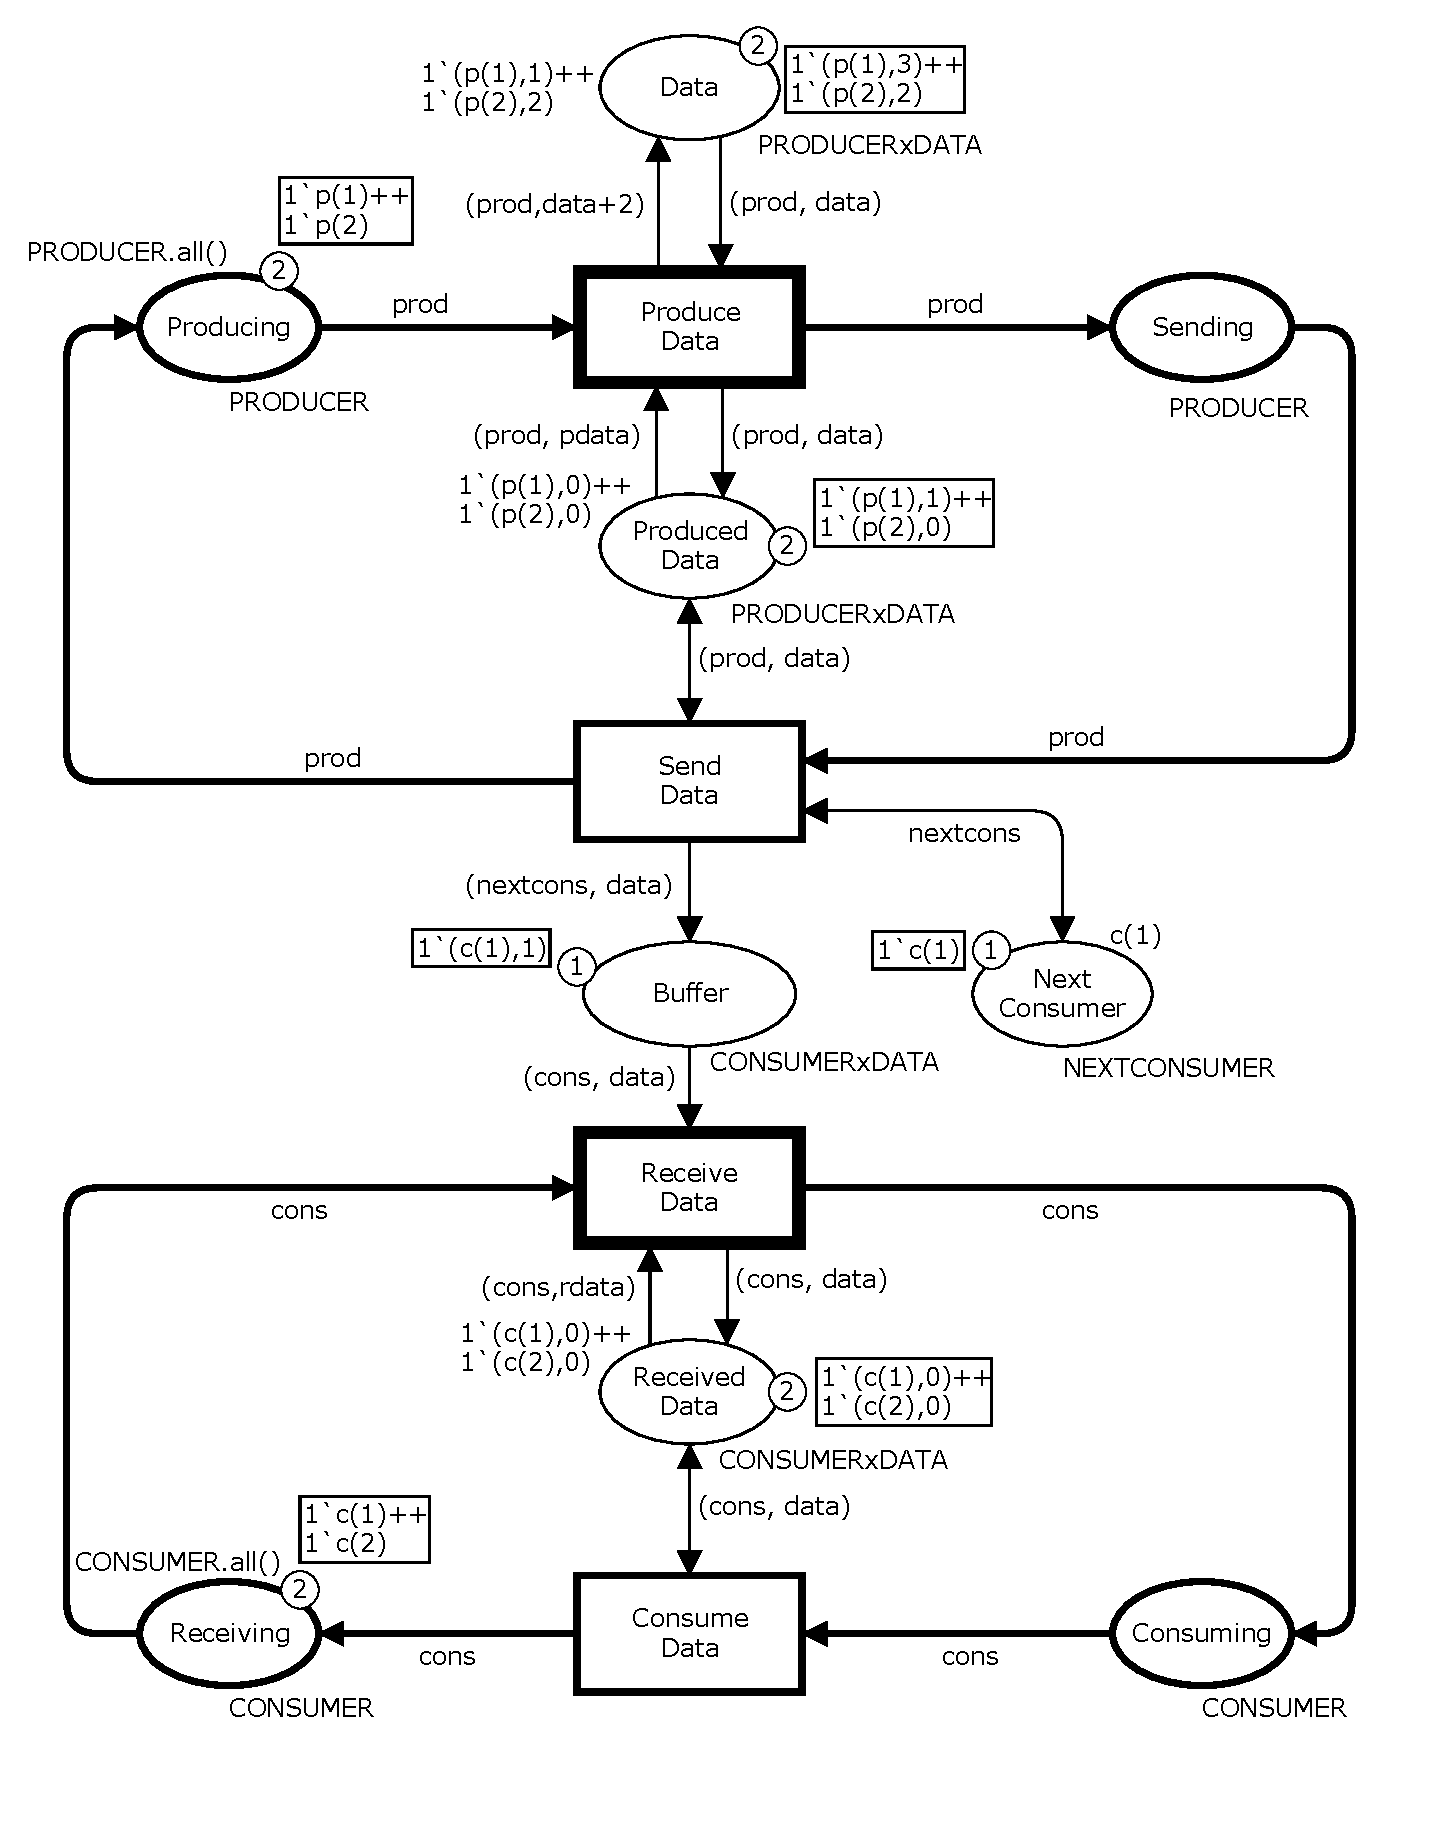
\includegraphics[scale=0.35]{background/graphics/SystemM2.eps}
\caption{The marking $M_2$ after the occurrence of \figitem{SendData}}
\label{fig:systemmoduleM2}
\end{figure}

\subsection{Concurrency and Conflict}
Two binding elements are in conflict if they are both enabled, but the occurrence of one of them removes a token also needed by the other binding element. In the marking $M_2$ there are three binding elements enabled: \\*
\newline
$PD_1$ = (\figitem{ProduceData}, \code{<prod=p(1),data=3>})\\*
$PD_2$ = (\figitem{ProduceData}, \code{<prod=p(2),data=1>})\\*
$SD_1$ = (\figitem{SendData}, \code{<cons=c(1),data=1>})\\*
\newline
The first two binding elements represent a producer producing some data and the last binding element represents a consumer receiving some data. All these binding elements can occur \emph{concurrently}, i.e., in parallel, thus there are no conflicts here. The producer and consumer runs concurrently since two binding elements, where one of the binding elements include a transition from the producer part of the model and the other binding element includes a transition from the consumer part of the model, are never in conflict. This is because no places in the model are input places for both transitions in the producer and consumer part of the model. 

The occurrence of binding element $SD_1$ leads to the marking $M_3$ shown in Fig. \ref{fig:systemmoduleConsumerM3}. The data item has been removed from the buffer and the transition \figitem{ReceiveData} is no longer enabled as explained above. The consumer \emph{1} is now ready to consume the received data.

\begin{figure}[b!]
\centering
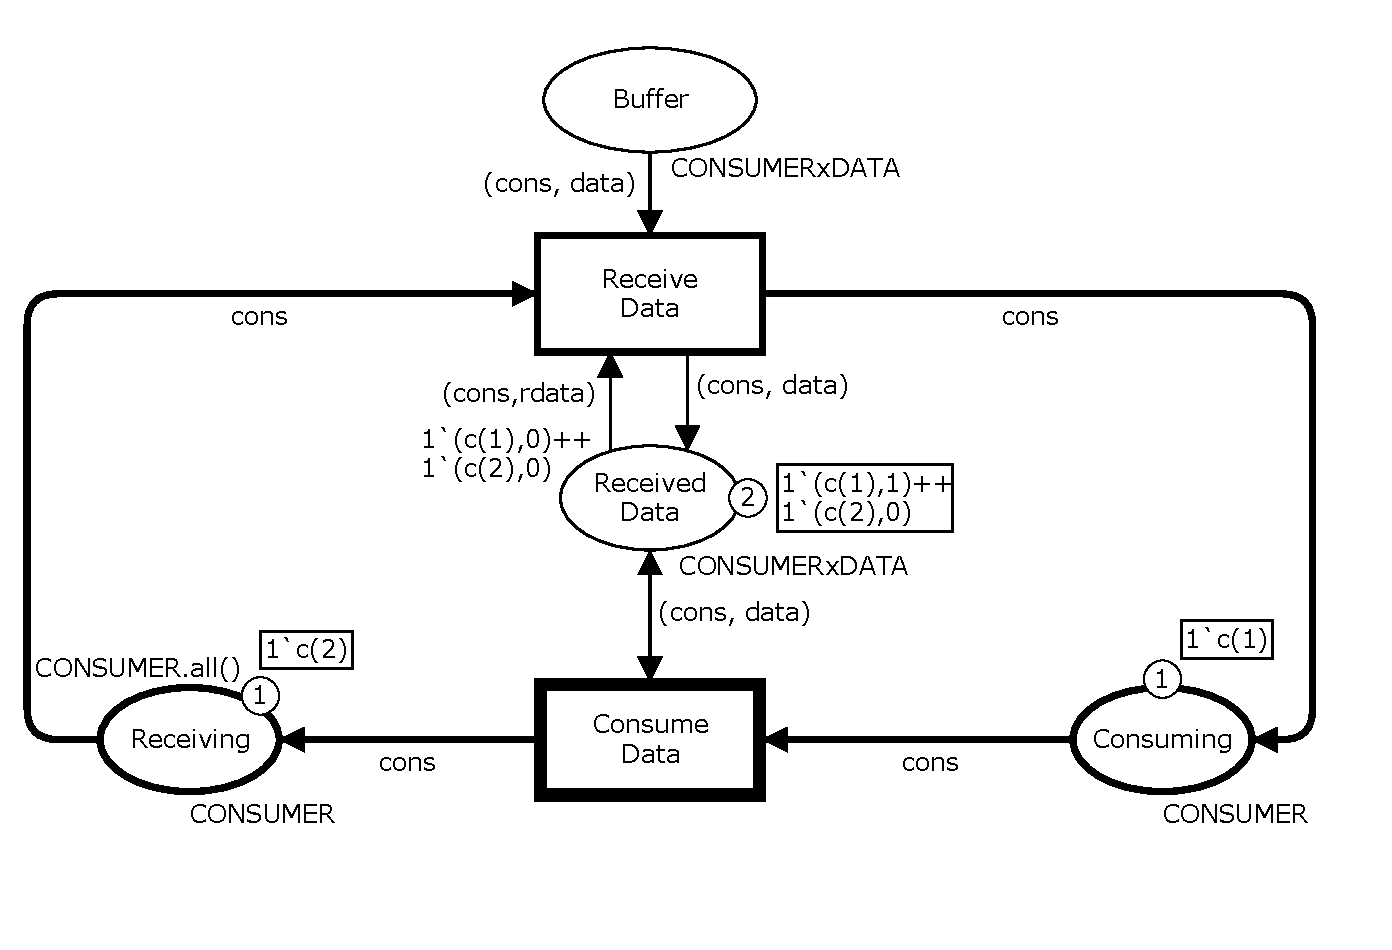
\includegraphics[scale=0.4]{background/graphics/SystemConsumerM3.eps}
\caption{The consumer part of the model in marking $M_3$}
\label{fig:systemmoduleConsumerM3}
\end{figure}


\subsection{Guards}
\label{subsec:guards}
Transitions are also allowed to have a guard which is a list of boolean expressions. A transition is only enabled if the guard expression evaluates to \emph{true} in the binding, thus putting an additional constraint on the transition. As an example of a guard consider the modified transition \figitem{ReceiveData} in Fig. \ref{fig:partsystemwithguard}. The guard of the transition \figitem{ReceiveData} is the boolean expression in the square brackets. It ensures that \code{c(1)} only receives even integers, whereas other consumers can receive both odd and even integers. This is done by first checking whether the \code{cons} variable is bound to the value \code{c(1)} and if so whether the variable \code{data} is bound to an even integer. \code{true} is returned for other values of the \code{cons} variable indicating no constraint on the enabling of the transition for these consumers.

\begin{figure}
\centering
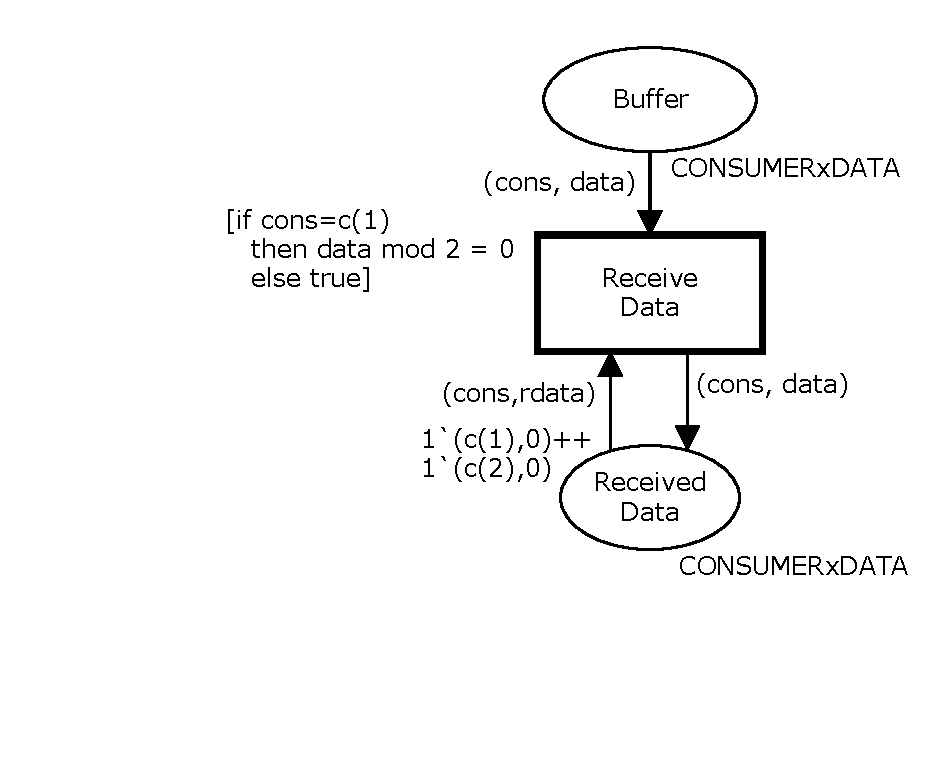
\includegraphics[scale=0.35]{background/graphics/PartSystemWithGuard.eps}
\caption{A guard constraining the enabling of the transition \figitem{ReceiveData}}
\label{fig:partsystemwithguard}
\end{figure}
